\section{Application Context}

The app is to be developed to provide a proof-of-concept for the framework.
Basic tasks of the app include showing off the capabilities of the framework, proving the implementation, and as an example on how to utilize the framework.

The app will be developed for Android 4 and above, although the framework will be independent from any Android version.
The app will force landscape view as it offers the more natural layout for the layout of the app.
Apart from OpenCV for the framework, the app shall have no further dependencies on further 3rd party tools.
This should ensure a clean and fast code for the application.

The app should be capable of running smoothly on a Tegra 3 processor\footnote{See: \url{http://www.nvidia.com/object/tegra-3-processor.html}.}.
The development device is the Transformer Prime, a 10'' tablet from ASUS\footnote{See: \url{http://eee.asus.com/en/transformer-prime/features}.}.
This means that the app should run smoothly on a 1.6Ghz Quadcore ARM processor rendering to a 1280 by 800 pixel screen.

\section{System Tasks}

In this section, we will take a look at the various tasks the final app should be capable of doing.
Note that we differentiate between required tasks (meaning tasks that should reliably and completely work for the app to be considered done) and optional tasks (tasks that might be included, depending on time and scope of their implementation).

\subsection{Required Tasks}

\begin{tabulary}{\textwidth}{L || L}
View Camera & The user should, upon opening the app, be confronted with the view of the live camera feed. By default, if a marker is detected, a simple 3d coordinate marker is shown in place of an object. \\
\hline
Load Model & Load and prepare a 3d model to be viewed in the camera feed on top of the marker. Any model in a recognized format should be selectable as a file from a file browser. \\
\hline
Modify Model & This task shall allow the user to change basic properties such as rotation and scale of a loaded object.\\
\hline
Unload Model & Unload a model, returning the view to the standard 3d coordinate marker on top of the marker (if detected). Unloading a model can also be achieved by loading a new one to replace it. \\
\hline
Change Settings & Allows the user to modify the frames per second to render the output, how often to update the frame, and the visual quality of the video feed on which the marker detection is run. Should enable the app to be adapted to run on a wide variety of devices.\\
\hline
Toggle Debugging Information & If desirable, the user can toggle a debugging view to be rendered on top of the feed. This should offer detailed information on the shown view, marker detection, and any other factors. \\
\hline
Screenshot & As Android does not offer a screenshot tool by default, an option to capture the feed shall be provided. \\
\end{tabulary}

\subsection{Optional Tasks}

This section represents tasks that could be added but might not be.
Any feature that does not make the final app is to be taken as a suggestion for possible future expansion.

\begin{tabulary}{\textwidth}{L || L}
Marker Definition & If possible, the user can load any recognized picture to be used as a marker beyond the default one. Certain properties will most likely be required of the picture however. \\
\hline
Modify Model & Further options such as toggling the rendering of a wireframe or textures. Future work might even include shader control or blending options for transparency or blur.\\
\hline
Multiple Tracker Support & Enable the app to track multiple markers at once and render their objects simultaneously.\\
\hline
Primitive Objects & Allow basic text or pictures to be used directly as an object without having to build them manually in a 3d modeling program. This feature would enable fast prototyping for text- and picture-based AR.\\
\hline
Camera Chooser & For devices that have multiple cameras, allow the user to choose which one to use as source for the live view and the rendering.\\
\end{tabulary}

\section{Dialog Structure}

Figure \ref{fig:dialog_structure} shows a graph of the usage flow in the app graphical user interface.
Note that apart from the layout change from just the main screen to the screen with the menu displayed at the right border, all sub-menus are displayed in-place to the original menu.
This allows the main purpose of the app, namely the rendering of AR, to always be in the focus of the user.
This enables rapid and direct feedback to any changes the user does within the menus.

\begin{figure}
	\centering
	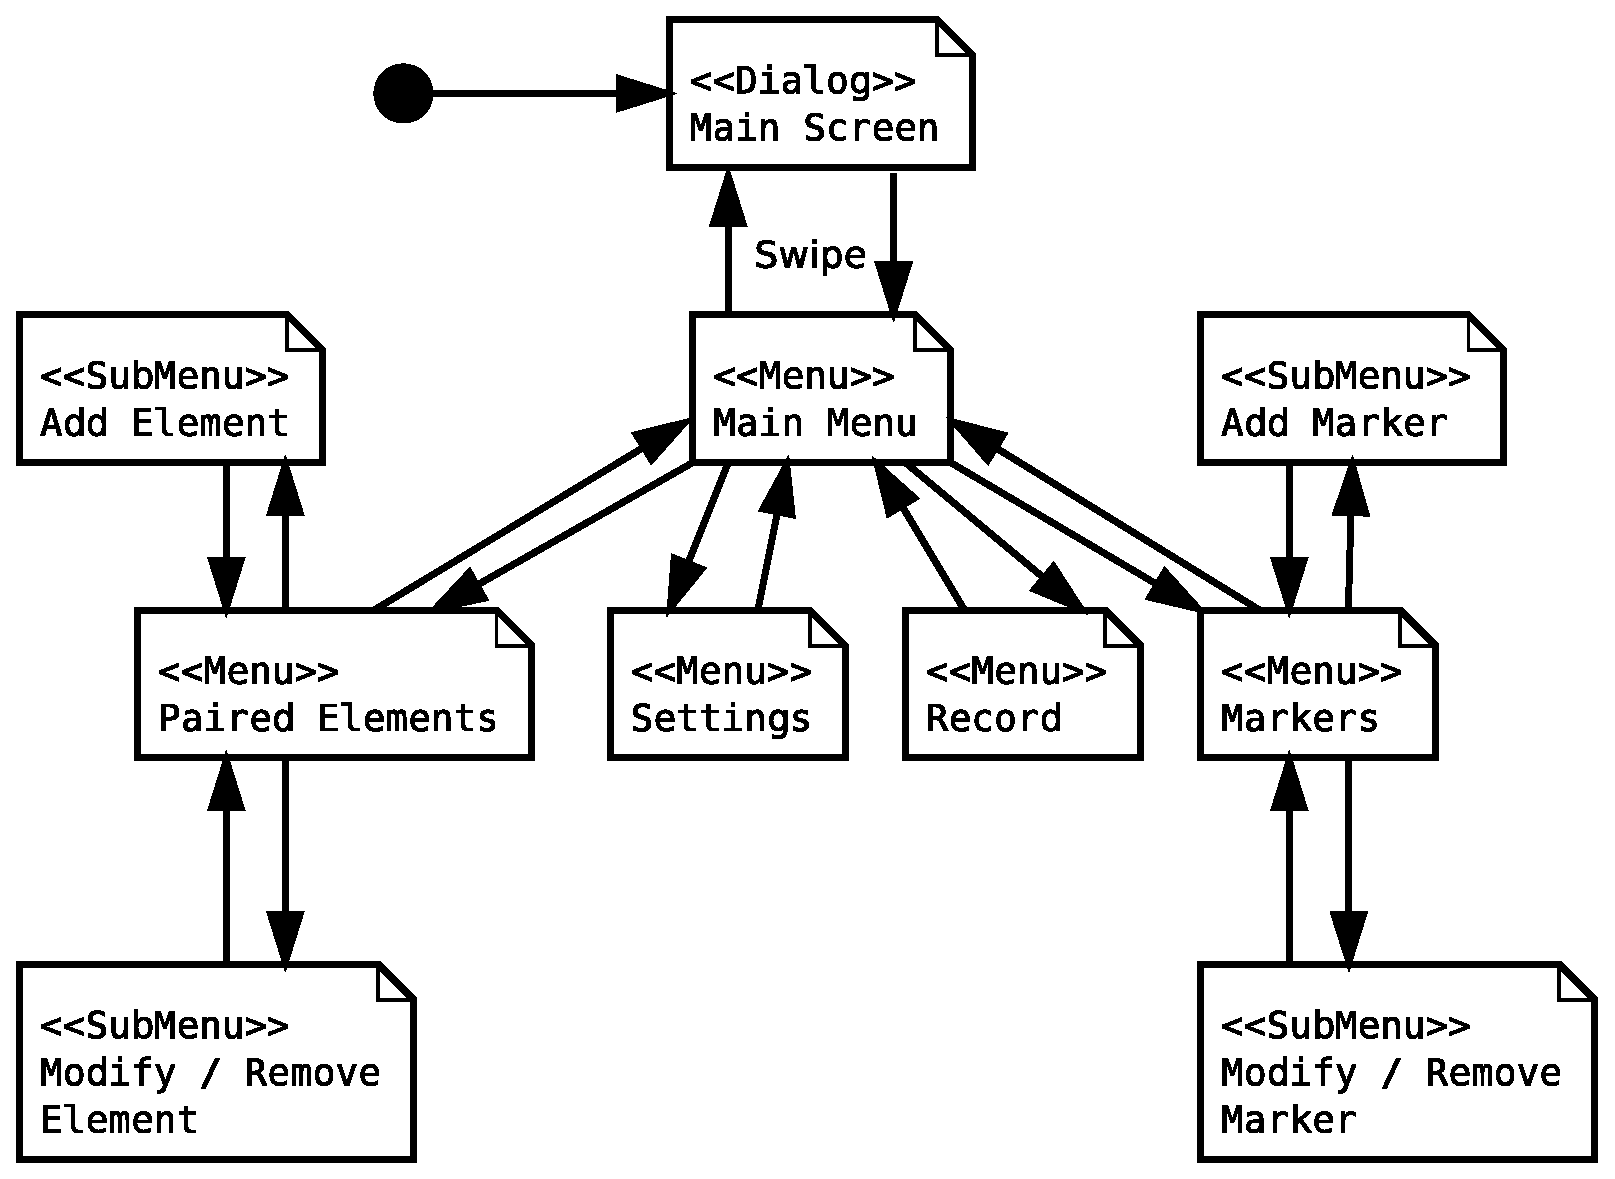
\includegraphics[width=10cm]{img/dialogs.eps}
	\caption[App Dialog Structure.]{Overview of the dialog structure of the app. Except where otherwise noted, all actions from one dialog to another are a simple touch.}
	\label{fig:dialog_structure}
\end{figure}

\section{Mockups}

\begin{figure}
	\centering
	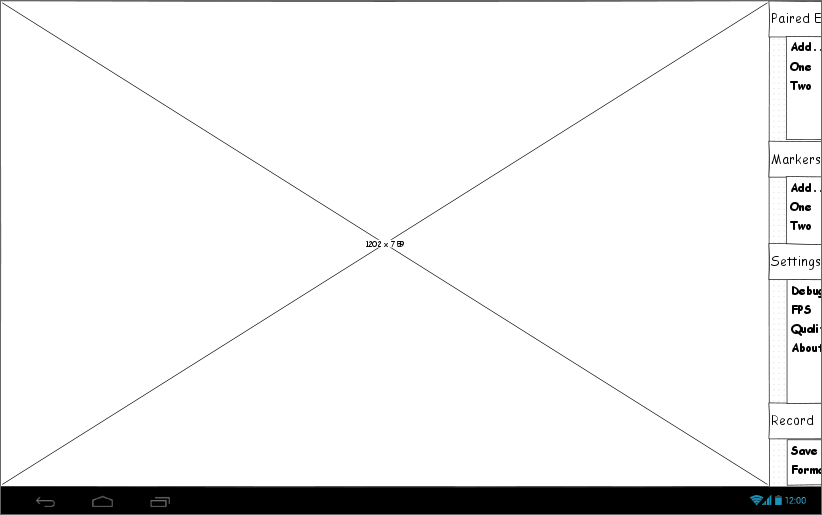
\includegraphics[width=15cm]{img/main_nomenu.png}
	\caption[Start screen mockup.]{Mockup of how the start screen of the final app might look. Note the menu partially hidden to the right, the rendered axes, and the green status light signifying that the marker is being read with a high confidence.}
	\label{fig:main_nomenu}
\end{figure}

Upon starting the app on a capable device, the app presents itself as shown in Figure \ref{fig:main_nomenu}.
This is effectively the start screen from where all the interaction takes place.

The green light in the top left shows that the app is detecting the marker with a high confidence, meaning that there are no large uncertainties.
If the marker is too warped or partially covered, the light switches to red.
If the app can still detect the marker but is having difficulties, the light switches to orange.
This mechanism is meant to offer fast and accurate feedback to the detection capability.
Another method of direct feedback is the already displayed axis-object.
This is meant to offer fast feedback to the orientation and scaling of the coordinate space to the user before a custom object is displayed.
The visibility of the axis-object can be toggled in the settings.

The menu on the right can be swiped in to be fully displayed.
The four main points are <Paired Elements>, <Markers>, <Settings>, and <Record>.

TODO: Add mockup.

<Paired Elements> lists the current paired marker-object pairs that the app can detect.
From here, the user can modify existing pairs by touching them, which opens a new menu in place with options pertaining to that pair, including its removal.
Adding new pairs is done via the <Add> button at the top, displaying a menu to select the marker and object to pair.

TODO: Add mockup.

<Markers> lists the available markers and provides options for organizing them.
Again, touching a marker opens an in-place menu with options.
Adding new markers, either by loading a picture, using a default, or taking a picture from the camera, can be done via the <Add> button.

TODO: Add mockup.

<Settings> is just that.
Here, the user can change app-specific settings such as video resolution, directories, debugging information, and more.

TODO: Add mockup.

<Record> allows the user to record the current rendering, either as a picture or possibly as a video.
The options beneath this item are for controlling those features.
